\subsection{LED-Ansteuerung} \label{LED-Ansteuerung}
Die LEDs des Baseboards werden wie im Skript beschrieben mit einem PWM Timer über DMA angesteuert, um den Prozessor zu entlasten. Mit dieser Methode müssen allerdings im DMA-Buffer pro LED 24 32-Bit Integers gespeichert werden. Demnach ist eine Ansteuerung der Matrix mit 960 LEDs aufgrund des begrenzten RAM des Controlles so nicht möglich. Deshalb wurde zur Ansteuerung die SPI-Peripherie des µC verwendet. 
\begin{figure}[H]
    \centering
    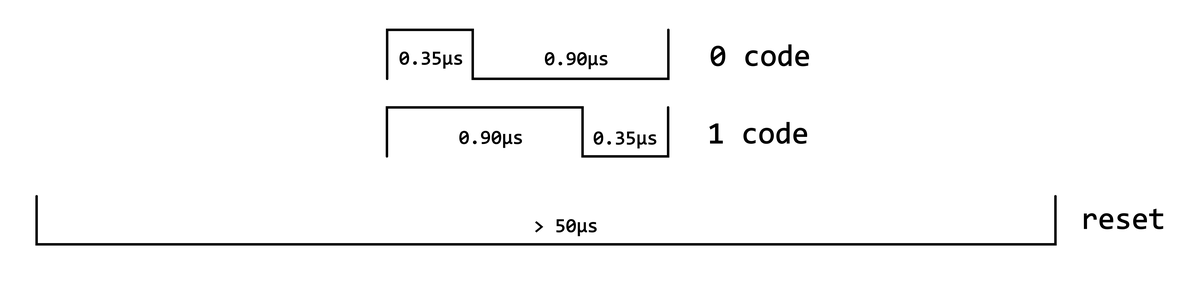
\includegraphics[page=1,width=0.85\textwidth]{images/ws2812b-timings.png} 
    \caption{Timings für die WS2812 LEDs \cite{ws2812_SPI}}
    \label{fig:ws2812b-timings}
\end{figure}
\noindent Um die timings für die LEDs zu generieren (Abb. \ref{fig:ws2812b-timings}), wurde mit 8 SPI-Bits pro Bit für das WS2812-Protokoll eine “0” als 10000000 und eine “1” als 11111100 codiert. Mit einem Prescaler für die SPI-Frequenz von 16 und einer Taktrate von 84 MHz ergibt sich eine Bitrate von 5,25 Mb/s. Da die LEDs sehr tolerant gegenüber Unterschieden im timing sind, funktionieren sie von ca. 3 bis 6 Mb/s. Durch das Nutzen des SPI-Busses mit 8 Bit pro WS2812-Bit wurde so die RAM-Auslastung auf 1/4 gegenüber der PWM-Methode verkleinert. Die Daten werden per DMA an die SPI-Peripherie übermittelt. Der Buffer wird zyklisch an die LEDs gesendet, sodass lediglich in den Buffer geschrieben werden muss und keine Aufrufen einer Funktion zur Aktualisierung der LEDs nötig ist.

\subsubsection{WS2812 DMA Library}
Die im Skript beschriebene Ansteuerung der LEDs des Baseboards wurde in einer Library realisiert. \\\\
\noindent \textbf{Konstanten:}
{\renewcommand\labelitemi{}
\begin{itemize}[leftmargin=*]
    \item \texttt{WS2812\_DMA\_*}: Verschiedene Konstanten, die die Anzahl von LEDs, Buffergrößen und die timings für die WS2812 LEDs konfigurieren.
\end{itemize}
}

\subsubsection*{Typen:}
{\renewcommand\labelitemi{}
\begin{itemize}[leftmargin=*]
    \item \texttt{PixelRGB\_t}: Eine union, die ein RGB-Pixel mit drei 8-Bit Farbkomponenten oder einen einzelnen 32-Bit Wert, für einfache Farbänderung enthält.
\end{itemize}
}
\begin{lstlisting}[style=CStyle]
typedef union
{
  struct
  {
    uint8_t b; /* blue */
    uint8_t r; /* red */
    uint8_t g; /* green */
  } c; /* color */
  uint32_t data; /* 32-bit for alignment */
} PixelRGB_t;
\end{lstlisting}

\subsubsection*{Globale Variablen}
{\renewcommand\labelitemi{}
\begin{itemize}[leftmargin=*]
    \item \texttt{WS2812\_DMA\_HANDLE}: Die \texttt{TIM\_HandleTypeDef} für des PWM timers.
    \item \texttt{ws2812\_DMA\_buffer}: DMA Buffer
    \item \texttt{ws2812\_DMA\_buffer\_ptr}: Pointer zum DMA Buffer
    \item \texttt{ws2812\_DMA\_pixels}: Ein Array vom Typ \texttt{PixelRGB\_t}, welcher die Farbwerte von jeder LED enthält.
\end{itemize}
}

\subsubsection*{Funktionen:}
{\renewcommand\labelitemi{}
\begin{itemize}[leftmargin=*]
    \item \texttt{void ws2812\_DMA\_init(void)}: Initialisiert den DMA Buffer mit dem Wert 0 (Schwarz) für jede LED.
    \item \texttt{void ws2812\_DMA\_write(PixelRGB\_t* pixel)}: Schreibt Farbdaten für einen einzelnen Pixel in den DMA Buffer.
    \item \texttt{void HAL\_TIM\_PWM\_PulseFinishedCallback(TIM\_HandleTypeDef *htim)}: Callbackfunktion, welche aufgerufen wird, wenn alle Daten aus dem DMA Buffer per PWM ausgegeben wurden. Stoppt den PWM timer.
    \item \texttt{void HAL\_TIM\_PeriodElapsedCallback(TIM\_HandleTypeDef *htim)}: Callbackfunktion für einen Timer zur Animation der LEDs.
\end{itemize}
}

\subsubsection{WS2812 SPI Library}
Die in \ref{LED-Ansteuerung} beschriebene Ansteuerung der LEDs der Matrix wurde in einer Library realisiert. \\\\
\noindent \textbf{Konstanten:}
{\renewcommand\labelitemi{}
\begin{itemize}[leftmargin=*]
    \item \texttt{WS2812\_SPI\_*}: Verschiedene Konstanten, die die Anzahl von LEDs, Buffergrößen und die timings für die WS2812 LEDs konfigurieren.
    \item \texttt{WS2812\_SPI\_FILL\_BUFFER}: Ein Macro, welches den SPI Buffer mit den Farbdaten für die WS2812 LEDs füllt.
\end{itemize}
}

\subsubsection*{Typen:}
{\renewcommand\labelitemi{}
\begin{itemize}[leftmargin=*]
    \item \texttt{PixelRGB\_t}: Eine union, die ein RGB-Pixel mit drei 8-Bit Farbkomponenten oder einen einzelnen 32-Bit Wert, für einfache Farbänderung enthält.
\end{itemize}
}

\subsubsection*{Globale Variablen}
{\renewcommand\labelitemi{}
\begin{itemize}[leftmargin=*]
    \item \texttt{WS2812\_SPI\_HANDLE}: Die \texttt{SPI\_HandleTypeDef} der SPI Peripherie.
    \item \texttt{ws2812\_SPI\_buffer}: Der Buffer für die SPI Daten.
\end{itemize}
}

\subsubsection*{Funktionen:}
{\renewcommand\labelitemi{}
\begin{itemize}[leftmargin=*]
    \item \texttt{void ws2812\_SPI\_init(void)}: Initialisiert den DMA Buffer mit dem Wert 0 (Schwarz) für jede LED und startet die SPI DMA Übertragung.
    \item \texttt{void ws2812\_SPI\_pixel(uint8\_t x, uint8\_t y, PixelRGB\_t* color)}: Setzt den Farbwert eines Pixels an den entsprechenden Koordinaten.
    \item \texttt{void ws2812\_SPI\_pixel\_all(PixelRGB\_t* color)}: Setzt alle Pixel auf den gegebenen Farbwert.
    \item \texttt{void ws2812\_SPI\_draw(PixelRGB\_t** picture, uint8\_t width, uint8\_t height)}: Setzt die LEDs auf die im zweidimensionalen Array \texttt{picture} gepseicherten Farbwerte.
    \item \texttt{void HAL\_SPI\_TxCpltCallback(SPI\_HandleTypeDef* hspi)}: Callbackfunktion, welche aufgerufen wird, wenn alle Daten aus dem DMA Buffer über SPI ausgegeben wurden. Startet die SPI DMA Übertragung erneut.
\end{itemize}
}

\subsubsection*{Verwendung des Lookup Tables in der LED-Ansteuerung}

Ein wesentliches Element der Ansteuerung der LEDs der Matrix ist der Einsatz eines Lookup Tables, der in \texttt{lookup\_table.c} definiert und initialisiert wird. Der Lookup-Table bildet Koordinaten (x, y) auf einen linearen Index ab, der den Positionen der LEDs in der seriellen Anordnung in der Matrix entspricht.

\begin{lstlisting}[style=CStyle]
typedef struct {
    uint16_t rows;
    uint16_t cols;
    uint16_t** index;
} LookupTable;
\end{lstlisting}

Innerhalb von \texttt{ws2812\_SPI.c} wird der Lookup-Table genutzt, um die Position jeder LED in der Matrix zu bestimmen und die entsprechenden Farbdaten korrekt im SPI-Datenpuffer zu positionieren. Dies ermöglicht es, spezifische LEDs basierend auf ihren Koordinaten anzusteuern und komplexe Muster oder Animationen auf der LED-Matrix zu erzeugen.

\begin{lstlisting}[style=CStyle]
void ws2812_SPI_pixel(uint8_t x, uint8_t y, PixelRGB_t* color) {
    uint8_t* ptr = &ws2812_SPI_buffer[24 * lookupTable.index[y][x]];
    // Setze Farbdaten im Buffer...
}
\end{lstlisting}

\subsection{Labyrinth} \label{Labyrinth}
In diesem Abschnitt wird eine Software zur Generierung und Lösung von Labyrinthen auf einer LED-Matrix vorgestellt. Die Matrix besteht aus 40x24 WS2812 LEDs. Es wird eine Paketdrohne simuliert, die Pakete innerhalb eines virtuellen Labyrinths transportiert. Das Labyrinth wird dabei dynamisch generiert und der Start- und Zielpunkt hängt von der Lage des Nachbarteams und der Zustellrichtung ab. Auf der Nordseite der Matrix befindet sich das Nucleoboard mit Lager sowie Inbound- und Outbound-Punkten. In den anderen Himmelsrichtungen können sich Nachbarteams befinden, von denen Pakete empfangen oder an die Pakete gesendet werden können.

Das Ziel der Software ist es, den Pfad der Paketdrohne durch das Labyrinth zu berechnen und zu visualisieren. Dabei werden die Drohne und das transportierte Paket auf der LED-Matrix animiert dargestellt. Die Drohne folgt einem vorgegebenen Pfad vom Startpunkt zum Zielpunkt, um das Paket effizient zu liefern. Die Farbe des Pakets wird dabei durch eine vorgegebene Paketfarbe repräsentiert, die im Verlauf der Animation sichtbar ist.

Die Software besteht aus mehreren Komponenten, wie der Generierung des Labyrinths, der Lösung des Labyrinths mittels eines Pfadsuchalgorithmus und der Darstellung der Drohnenbewegung auf der LED-Matrix. Diese Dokumentation beschreibt die Schlüsselfunktionen der einzelnen Quelldateien und erläutert die zugrundeliegenden Konzepte und Algorithmen.

\subsection{Pseudozufallszahlengenerator (PRNG)}

Der Pseudozufallszahlengenerator, implementiert in \texttt{prng.c}, spielt eine zentrale Rolle in der Generierung von Labyrinthen und der Entscheidungsfindung innerhalb der Software. Er nutzt eine vordefinierte Liste von Zahlen aus \texttt{numbers.c}, um eine Sequenz von scheinbar zufälligen Werten zu erzeugen, die dennoch reproduzierbar und vorhersagbar sind.

\subsubsection{Implementierung des PRNG}

Die Datei \texttt{prng.c} definiert einen Pseudozufallszahlengenerator mithilfe einer Struktur, die einen Zeiger auf ein Array von Zahlen, einen Index und die Größe des Arrays enthält. Diese Struktur ermöglicht es, durch die Zahlenliste zu iterieren und „zufällige“ Werte für die Labyrinthgenerierung und -navigation zu liefern.

\begin{lstlisting}[style=CStyle]
typedef struct {
    int* num; /* Zeiger auf Array von vordefinierten Zahlen */
    int ind;  /* Aktueller Index im Array */
    int size; /* Groesse des Arrays */
} PseudoRNG;
\end{lstlisting}

Die Initialisierung des PRNG erfolgt durch die Funktion \texttt{initPRNG}, die das Array von Zahlen, seinen Index und die Größe setzt. Die Funktion \texttt{getRand} wird verwendet, um den nächsten Wert aus dem Array zu extrahieren, wobei der Index nach jeder Operation inkrementiert wird.

\subsubsection{Nutzung der Zahlenliste aus \texttt{numbers.c}}

Die Zahlenliste in \texttt{numbers.c} enthält eine statisch definierte Sequenz von Werten, die als Grundlage für den PRNG dienen. Diese Liste ermöglicht eine effiziente Umsetzung eines pseudozufälligen Zahlengenerators.

\begin{lstlisting}[style=CStyle]
int numbers[] = {57341, 32796, ..., 29396};
\end{lstlisting}

\subsection{Generierung des Labyrinths}

Die Generierung des Labyrinths wird hauptsächlich durch die Funktionen innerhalb der Datei \texttt{maze.c} gesteuert, unterstützt durch globale Definitionen und Hilfsfunktionen aus anderen Quelldateien wie \texttt{numbers.c} und \texttt{prng.c} für die Pseudo-Zufallszahlengenerierung.

\subsubsection{Strukturen in \texttt{maze.h}}

Für die Generierung und Handhabung des Labyrinths definiert die Datei \texttt{maze.h} mehrere zentrale Strukturen (`structs`), die sowohl die physikalischen Eigenschaften des Labyrinths als auch die Navigationspunkte innerhalb desselben repräsentieren. \\

\noindent \textbf{Point-Struktur}

Die `Point`-Struktur repräsentiert einen Punkt innerhalb des Labyrinths und enthält Koordinaten sowie Verknüpfungen zu vorherigen und nächsten Punkten, falls verwendet.

\begin{lstlisting}[style=CStyle]
typedef struct {
    int x; /* x-Koordinate */
    int y; /* y-Koordinate */
    struct Point *prev; /* Zeiger auf vorherigen Punkt im Pfad */
    struct Point *next; /* Zeiger auf naechsten Punkt im Pfad */
} Point;
\end{lstlisting}

\noindent \textbf{Maze-Struktur}

Die `Maze`-Struktur beschreibt das Labyrinth selbst. Sie enthält Informationen über die Dimensionen des Labyrinths (Anzahl der Reihen und Spalten), Start- und Endpunkte sowie das eigentliche Gitter, das die Struktur des Labyrinths repräsentiert.

\begin{lstlisting}[style=CStyle]
typedef struct {
    uint8_t rows;   /* Anzahl der Reihen im Labyrinth */
    uint8_t cols;   /* Anzahl der Spalten im Labyrinth */
    Point start;    /* Startpunkt */
    Point exit;     /* Zielpunkt */
    uint8_t** grid; /* 2D-Array, das das Labyrinth darstellt */
} Maze;
\end{lstlisting}

\noindent \textbf{Queue-Struktur}

Für die Speicherung und Verwaltung der zu durchsuchenden Punkte während der Labyrinthlösung wird eine `Queue`-Struktur verwendet, die eine Warteschlange implementiert. Sie ist insbesondere für die Implementierung der Breitensuche (BFS) relevant.

\begin{lstlisting}[style=CStyle]
typedef struct {
    Point* head; /* Zeiger auf den ersten Punkt in der Warteschlange */
    Point* tail; /* Zeiger auf den letzten Punkt in der Warteschlange */
    uint16_t size; /* Anzahl der Punkte in der Warteschlange */
} Queue;
\end{lstlisting}

\subsubsection{Der Generierungsprozess}

Die Labyrinthgenerierung beginnt mit der Initialisierung des Maze-Structs, indem die \texttt{initMaze} Funktion aufgerufen wird. Diese Funktion legt die Größe des Labyrinths fest und initialisiert das Gitter mit Wänden (\texttt{WALL}).

\begin{lstlisting}[style=CStyle]
void initMaze(Maze* maze, uint8_t rows, uint8_t cols, 
              uint8_t startX, uint8_t startY, 
              uint8_t exitX, uint8_t exitY) {
    maze->rows = rows;
    maze->cols = cols;
    // Weitere Initialisierungen...
}
\end{lstlisting}

Nach der Initialisierung beginnt der eigentliche Generierungsprozess, der eine Reihe von Schritten durchläuft, um Wege (\texttt{PATH}) im Labyrinth zu schaffen. Die Funktion \texttt{carveMaze} wird für jede Zelle des Labyrinths aufgerufen, beginnend bei der Startposition. Die Funktion wählt zufällig eine Richtung aus und versucht, in dieser Richtung zwei Zellen weit zu “graben” (Wege zu schaffen), vorausgesetzt, die Zielzelle und die dazwischenliegende Zelle sind beide Wände.

\begin{lstlisting}[style=CStyle]
void carveMaze(Maze* maze, uint8_t x, uint8_t y) {
    int dir = getRand(&rng) % 4; /* Zufaellige Richtung */
    // Versuche, in der gewaehlten Richtung zu graben
}
\end{lstlisting}

Die zufällige Auswahl der Richtung und das Überprüfen, ob ein Graben möglich ist, gewährleisten, dass das generierte Labyrinth sowohl zufällig als auch lösbar ist.

\subsubsection{Schlüsselkonzepte}

Ein Schlüsselkonzept in der Labyrinthgenerierung ist die rekursive Backtracking-Methode, die sicherstellt, dass das gesamte Gitter erkundet und ein lösbares Labyrinth erzeugt wird. Jeder Schritt der Generierung wählt zufällig eine neue Richtung, um die Vielfalt und Komplexität des Labyrinths zu erhöhen.

Das Ergebnis dieses Prozesses ist ein Labyrinth mit einem klaren Pfad vom Start zum Ziel, bereit für die Paketdrohne, um das Paket zu liefern. Die Visualisierung dieses Pfades und die Animation der Drohnenbewegung werden durch die nachfolgenden Schritte der Software unterstützt.

\subsection{Lösung des Labyrinths}

Nachdem das Labyrinth generiert wurde, besteht die nächste Herausforderung darin, einen Weg vom Startpunkt zum Ziel zu finden. Diese Aufgabe wird von der Funktion \texttt{solveMaze} in der Datei \texttt{maze.c} übernommen. Der Kern dieses Prozesses basiert auf dem Algorithmus der Breitensuche (Breadth-First Search, BFS), einem klassischen Suchalgorithmus, der für die Lösung von Labyrinthen besonders gut geeignet ist.

\subsubsection{Der Lösungsalgorithmus}

Die Breitensuche beginnt am Startpunkt des Labyrinths und erkundet systematisch alle benachbarten Zellen, bis der Zielpunkt gefunden wird. Dies geschieht durch die schrittweise Exploration aller von einer Zelle aus erreichbaren Nachbarzellen, wobei jede neu entdeckte Zelle in eine Warteschlange eingefügt wird. Die Zellen in der Warteschlange repräsentieren den aktuellen “Rand” der Erkundung. 

\begin{lstlisting}[style=CStyle]
void solveMaze(Maze* maze, Queue* path) {
    // Initialisierung der Warteschlange und Markierung des Startpunkts
    
    while (/* queue nicht leer */) {
        // Entferne das vorderste Element der Warteschlange
        // Ueberpruefe, ob das Ziel erreicht wurde
        // Fuege benachbarte, noch nicht besuchte Zellen der Warteschlange hinzu
    }
}
\end{lstlisting}

Jede Zelle wird dabei nur einmal besucht, um sicherzustellen, dass der Algorithmus den kürzesten Pfad zum Ziel findet.

\subsubsection{Schlüsselkonzepte}

Ein zentrales Konzept der Breitensuche ist die Verwendung einer Warteschlange zur Speicherung der zu erkundenden Zellen. Dies gewährleistet, dass die Zellen in der Reihenfolge ihrer Entdeckung bearbeitet werden, was für die Findung des kürzesten Pfads entscheidend ist. Die Implementierung der Warteschlange erfolgt über die in \texttt{queue.c} definierten Funktionen, die eine effiziente Handhabung der Ein- und Ausgabeoperationen ermöglichen.

Ein weiteres wichtiges Element ist die Markierung der besuchten Zellen, um sicherzustellen, dass der Algorithmus nicht in eine Endlosschleife gerät. Diese Markierungen helfen auch dabei, den zurückgelegten Pfad nachzuvollziehen, sobald das Ziel erreicht ist.

\subsubsection{Implementierungsdetails}

Die Implementierung der Breitensuche in \texttt{solveMaze} nutzt zusätzlich zu den Warteschlangenoperationen eine Reihe von Hilfsfunktionen, um benachbarte Zellen zu identifizieren und zu überprüfen, ob sie Teil des Lösungspfads sein können. Diese Überprüfungen beinhalten, ob eine Zelle bereits besucht wurde und ob sie eine Wand oder ein Pfad ist.

\begin{lstlisting}[style=CStyle]
// Beispiel: Hinzufuegen einer benachbarten Zelle zur Warteschlange
if (maze->grid[adjacentY][adjacentX] == PATH && !visited[adjacentY][adjacentX]) {
    enqueue(queue, adjacentX, adjacentY);
    // Markiere die Zelle als besucht
    visited[adjacentY][adjacentX] = true;
}
\end{lstlisting}

\subsubsection{Animation der Drohne auf der LED-Matrix}

Nachdem ein Pfad durch das Labyrinth gefunden wurde, wird die Bewegung der Paketdrohne auf der LED-Matrix animiert, um die Lieferung des Pakets visuell darzustellen. Die “Drohne” wird durch einen Pixel in der vorgegebenen Paketfarbe repräsentiert, welcher den gelösten Pfad entlang navigiert. \\

\noindent \textbf{Darstellung der Drohne}

Die Drohne wird als einzelner leuchtender Pixel auf der LED-Matrix dargestellt. Die Farbe dieses Pixels entspricht der Farbe des Pakets, was die Drohne visuell hervorhebt. Während die Drohne den Pfad entlangfliegt, wird ihre aktuelle Position auf der Matrix stetig aktualisiert, um die Bewegung entlang des Pfades zu simulieren. \\

\noindent \textbf{Visualisierung des Pfades}

Um den Pfad, den die Drohne zurücklegt, besser nachvollziehen zu können, werden bereits besuchte Zellen in einer dunkleren Version der Paketfarbe eingefärbt. Dies schafft einen visuellen Kontrast zwischen dem aktuellen Standort der Drohne und dem bereits zurückgelegten Weg. \\

\noindent \textbf{Implementierung der Animation}

Die Animation wird durch eine Schleife implementiert, welche den gefundenen Pfad Punkt für Punkt durchläuft und die LED-Farben entsprechend anpasst. Die Arrays \texttt{color} und \texttt{darkColor} speichern die Farben bzw. dunklere Versionen gemäß der Spezifikation der Paketfarben laut Aufgabenstellung.

\begin{lstlisting}[style=CStyle]
for (i = path.size - 1; i > -1; i--) {
    ws2812_SPI_pixel(path.p[i].x, path.p[i].y, &color[packageId]);
    HAL_Delay(ANIMATION_FRAMETIME_MS);
    ws2812_SPI_pixel(path.p[i].x, path.p[i].y, &darkColor[packageId]);
}
\end{lstlisting}
